\section{Experimental Setup}
\label{sec:eval}

\section{Evaluation}

Here we hijack an RDMA session and learn \emph{secret} data from a the remote
memory of an unsuspecting server. Then using a similar but slightly modified
version of the attack we inject write verbs and demonstrate that we can easily
write to exposed RDMAable memory. Figure~\ref{fig:tmp} is an example of what a
figure can be.

\begin{figure}[h]
    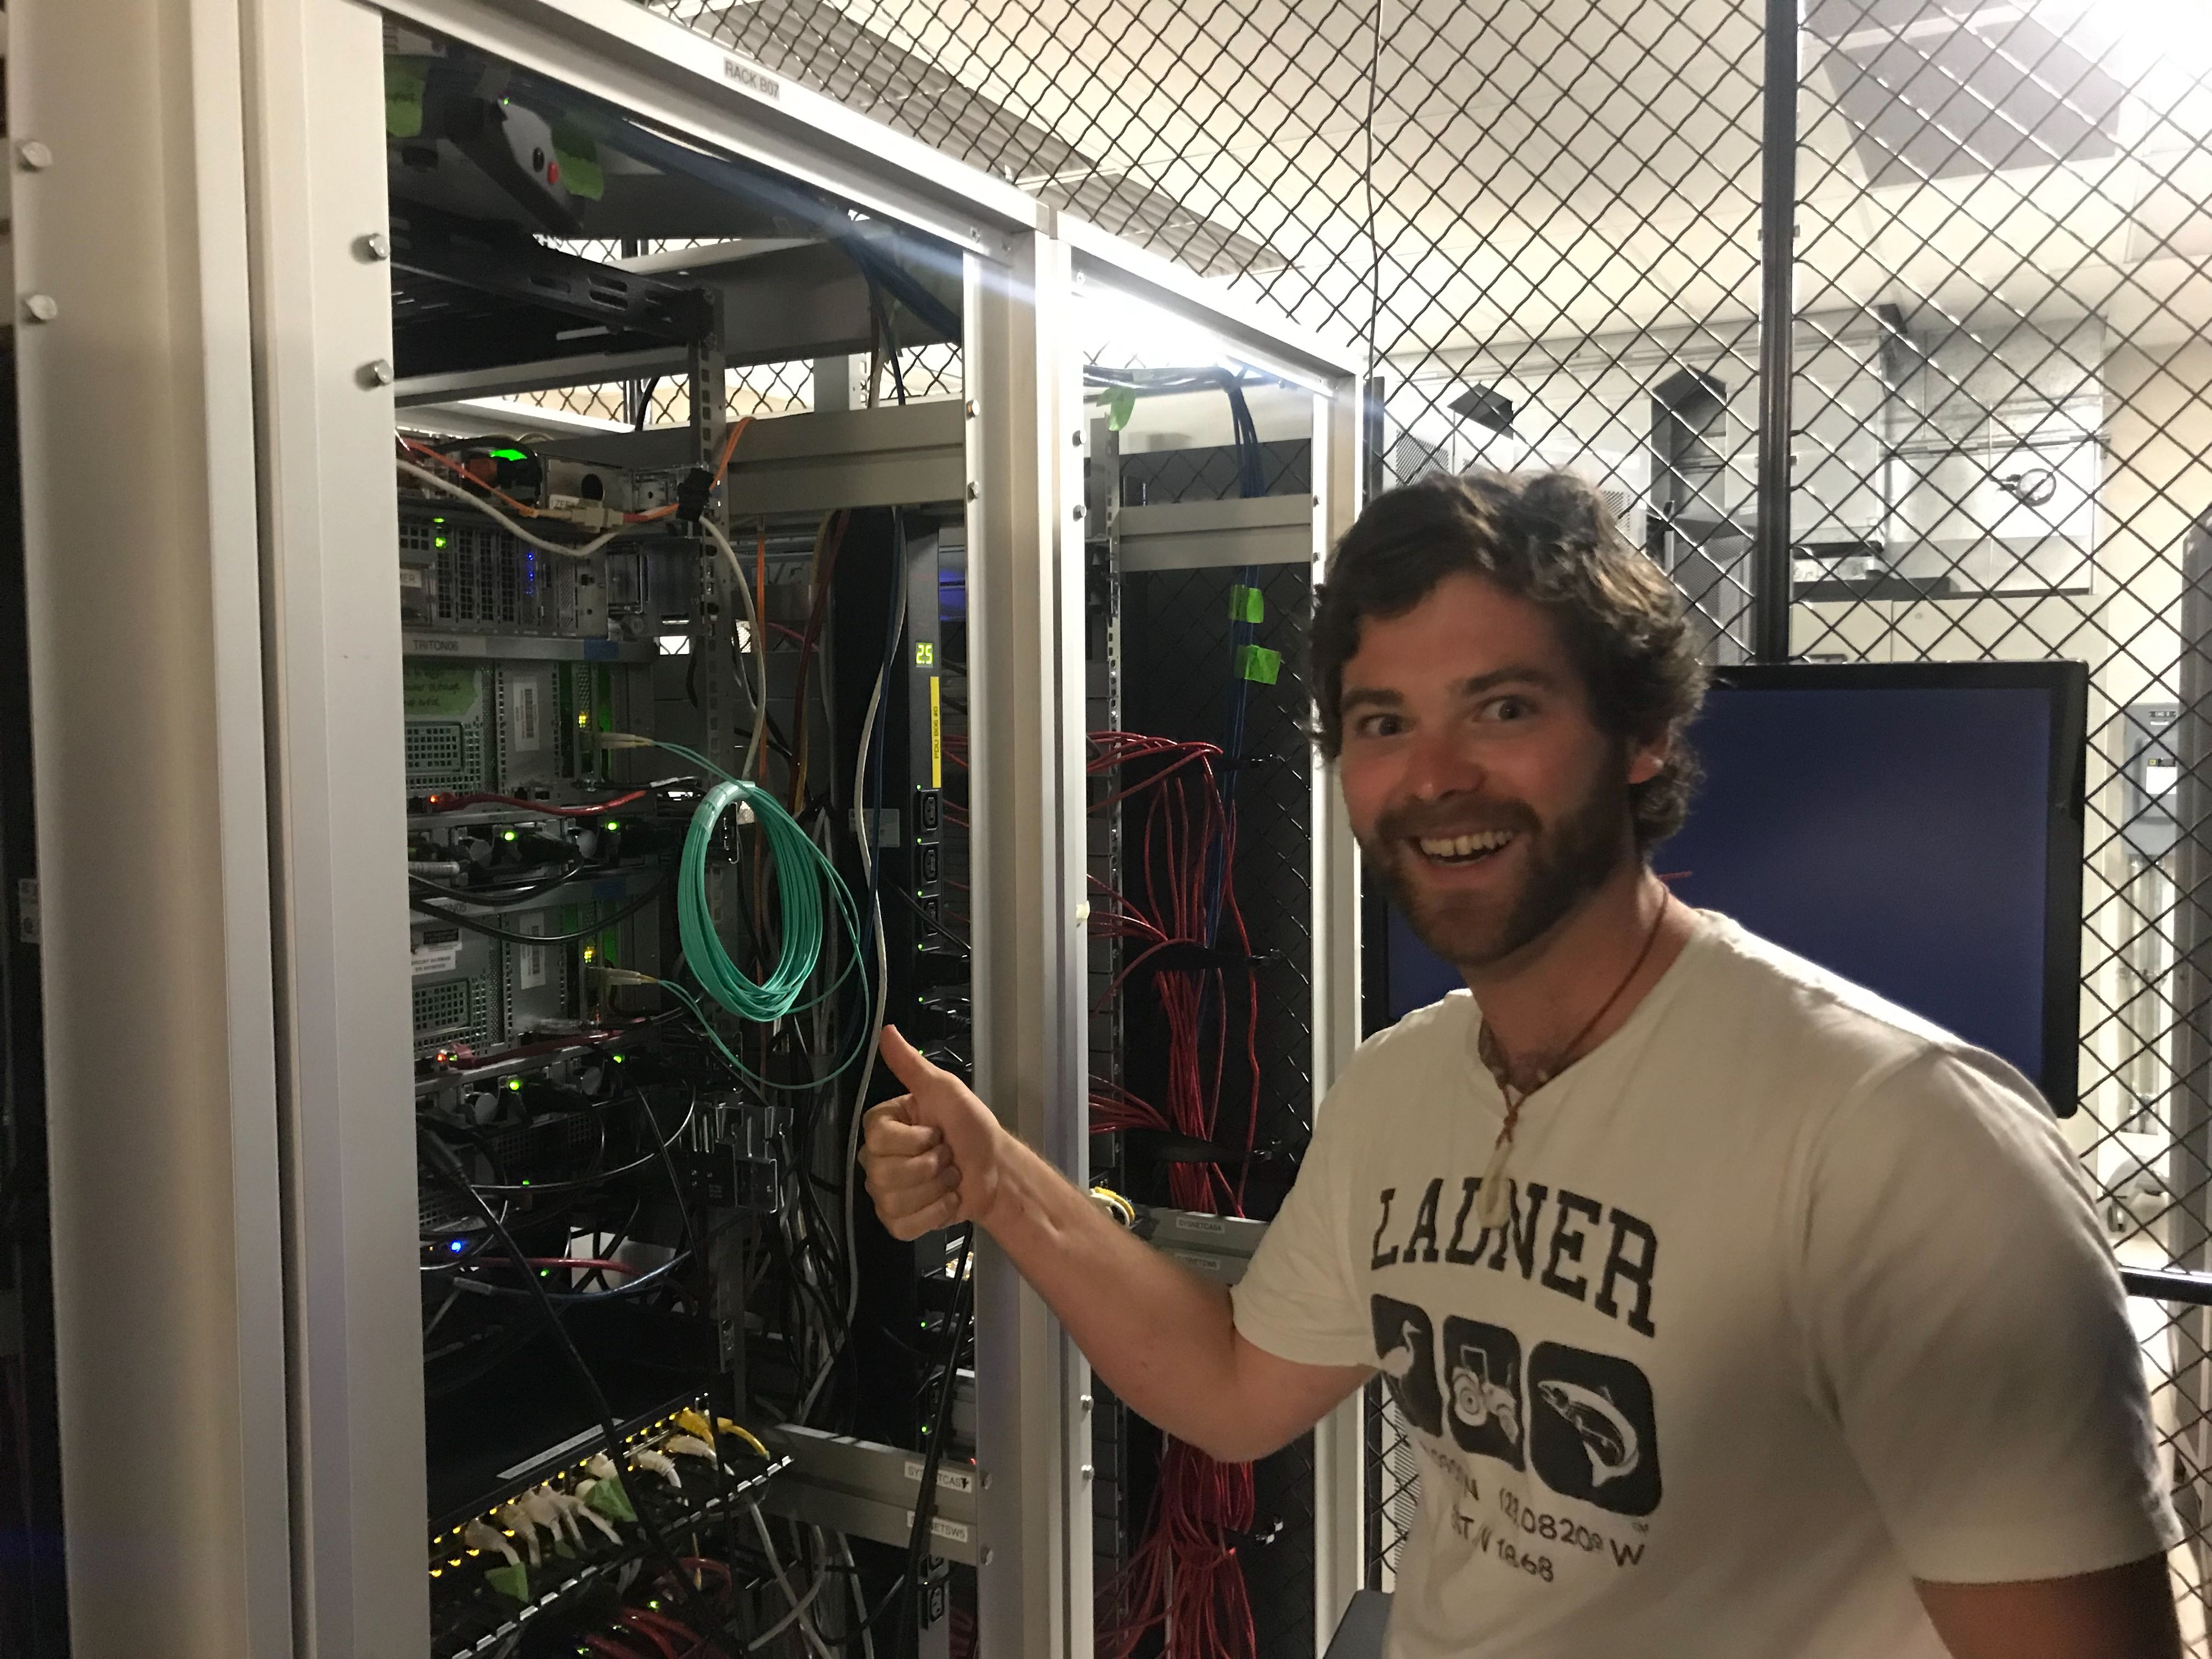
\includegraphics[width=0.5\textwidth]{fig/tmp.jpg}
    \centering
    \caption{My goodness this is a fantastic figure, it's so nice it could probably be used at a template for future figures.}
    \label{fig:tmp}
\end{figure}

\begin{table}
    \begin{tabular}{p{1.5cm}|p{1.5cm}|p{1.5cm}|p{1.5cm}}
        \hline
        \hline
    RDMA Variant & Sec prop & Verbs & Attack \\
        \hline
        RC & Seq Num & Read, Write, Send, Rec & Spoofing Seq \\
        \hline
        UC & & Read, Send, Rec & Read  \\
        \hline
        UD & Queue Pain Key & Send, Rec & \\
        \hline
    \end{tabular}
    \caption{A table roughly describing RDMA security primitives}
    \label{table:attacks}
\end{table}

